\documentclass{../template/Report}%方括号内写yuxi即生成预习报告\documentclass[yuxi]{../template/Report}
\settemplatedir{../template/}%设置模板路径

\exname{} %实验名称
\extable{} %实验桌号
\instructor{} %指导教师
\class{} %班级
\name{} %姓名
\stuid{} %学号

\nyear{} %年
\nmonth{} %月
\nday{} %日
\nweekday{} %星期几，e.g. \nweekday{三}
\daypart{}%上午/下午

\redate{} %如有实验补做，补做日期
\resitu{} %情况说明：

\begin{document}
\maketitle%输出封面

\section{预习报告（10分）}
（注：将已经写好的“物理实验预习报告”内容拷贝过来）

\subsection{实验综述（5分）}
（自述实验现象、实验原理和实验方法，包括必要的光路图、电路图、公式等。不超过500字。）

\subsubsection{实验目的}
研究铁磁材料的磁滞回线和基本磁化曲线，掌握利用示波器观测动态磁滞回线的原理与方法，通过测量材料在不同磁场下的磁化强度，计算并分析其磁学参数。

\subsubsection{实验原理}
铁磁性材料在外磁场 $H$ 作用下能被强烈磁化，介质中总磁感应强度 $B$ 为 $B = \mu_0(H+M) = \mu H$。由于铁磁质存在磁畴结构，其磁化过程不可逆，磁导率 $\mu$ 随磁场变化，且 $B$ 的变化滞后于 $H$，形成磁滞现象。
当磁场 $H$ 从零增加到饱和值 $H_s$，再减小至反向饱和并回到正向饱和时，$B-H$ 关系曲线构成闭合的磁滞回线。曲线与纵轴交点为剩磁 $B_r$，与横轴交点为矫顽力 $H_c$。各磁滞回线顶点的连线即为基本磁化曲线。

\begin{figure}[H]
    \centering
    % [图片占位：铁磁材料磁滞回线与基本磁化曲线]
    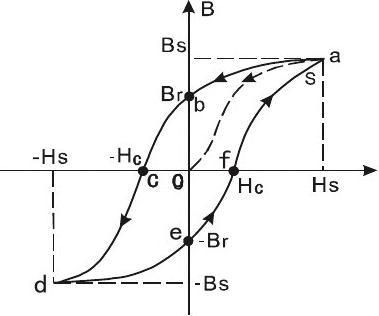
\includegraphics[width = 0.6\textwidth]{./figures/2/hysteresis_curve.png}
    \caption{铁磁材料的磁滞回线和基本磁化曲线}
    \label{fig:hysteresis_curve}
\end{figure}

本实验利用示波器显示磁滞回线，需将磁学量 $H$ 和 $B$ 转换为电压信号 $U_x$ 和 $U_y$。
对于磁场强度 $H$，由安培环路定理，原线圈电流 $I_1$ 产生磁场 $H = N_1 I_1 / L$。在回路中串联取样电阻 $R_1$，取其电压 $U_x = I_1 R_1$ 作为 $X$ 轴输入，则有：
\begin{equation}
    H = \frac{N_1}{L R_1} U_x
\end{equation}

对于磁感应强度 $B$，根据法拉第电磁感应定律，副线圈感应电动势 $\mathcal{E}_2 = -N_2 S \frac{dB}{dt}$。将副线圈接入 $RC$ 积分电路，在满足 $R_2 \gg \frac{1}{\omega C}$ 条件下，电容电压 $U_y$ 近似为：
\begin{equation}
    U_y \approx \frac{1}{C R_2} \int \mathcal{E}_2 dt = -\frac{N_2 S}{C R_2} B
\end{equation}
整理得 $B$ 与 $Y$ 轴电压的关系：
\begin{equation}
    B = -\frac{C R_2}{N_2 S} U_y
\end{equation}
实验时将 $U_x$ 和 $U_y$ 分别接入示波器 $CH1$ 和 $CH2$，在 $X-Y$ 模式下即可观测到由光点轨迹合成的磁滞回线。

\subsection{实验重点（3分）}
（简述本实验的学习重点，不超过100字。）

\begin{enumerate}
    \item 掌握铁磁材料磁化特性及磁滞回线、基本磁化曲线的物理意义。
    \item 理解将非电量 $H、B$ 转换为电量 $U_x、U_y$ 的测量电路原理。
    \item 准确测量回线关键点坐标，计算饱和磁感应强度 $B_s$、剩磁 $B_r$ 和矫顽力 $H_c$。
\end{enumerate}

\subsection{实验难点（2分）}
（简述本实验的实现难点，不超过100字。）

\begin{enumerate}
    \item 积分电路参数条件（$R \gg 1/\omega C$）及相位差对回线形状的影响与调节。
    \item 示波器定量测量的读数误差控制及 $X-Y$ 模式的操作。
    \item 根据实验数据绘制非线性的基本磁化曲线并进行准确的参数计算。
\end{enumerate}

\begin{fullreportonly}
    \section{原始数据（20分）}
    （将有老师签名的“自备数据记录草稿纸”的扫描或手机拍摄图粘贴在下方，完整保留姓名，学号，教师签字和日期。）

    \section{结果与分析}

    \subsection{数据处理与结果}

    \subsubsection{基本磁化曲线测量}

    实验中采用了硬磁材料作为待测样品，实验仪器的相关参数如下：励磁线圈匝数 $N_1=N_2=150$ 匝，样品的平均磁路长度 $L=\SI{0.130}{\meter}$，截面积 $S=\SI{1.24e-4}{\meter\squared}$。电路参数选取为采样电阻 $R_1=\SI{2.5}{\ohm}$，积分电阻 $R_2=\SI{10}{\kilo\ohm}$，积分电容 $C=\SI{3}{\micro\farad}$。

    我们在示波器上读取了峰峰值电压 $U_{xpp}$ 和 $U_{ypp}$，考虑到探头实际衰减比例，对原始读数进行了修正。随后依据安培环路定理与法拉第电磁感应定律，利用公式 $H = \frac{N_1}{2 L R_1} U_{xpp}$ 与 $B = \frac{C R_2}{2 N_2 S} U_{ypp}$ 将电压量换算为磁场强度 $H$ 与磁感应强度 $B$，并进一步计算相对磁导率 $\mu_r$。具体测量与计算结果详见表 \ref{tab:basic_curve}。

    \begin{table}[H]
        \centering
        \caption{基本磁化曲线测量与换算结果}
        \label{tab:basic_curve}
        \begin{tabular}{ccccccc} % 增加了一列，变为7列
            \toprule
            $U_{in}$ (\unit{\volt}) & $U_{x(pp)}$ (\unit{\volt}) & $U_{y(pp)}$ (\unit{\volt}) & $H$ (\unit{\ampere\per\meter}) & $B$ (\unit{\tesla}) & $\mu$ ($10^{-3}$\unit{\henry\per\meter}) & $\mu_r$ \\
            \midrule
            0.50                    & 0.1095                     & 0.0843                     & 25.26                          & 0.068               & 2.69                                     & 2141    \\
            1.00                    & 0.1995                     & 0.1625                     & 46.04                          & 0.131               & 2.84                                     & 2263    \\
            1.20                    & 0.2336                     & 0.1934                     & 53.91                          & 0.156               & 2.89                                     & 2301    \\
            1.50                    & 0.2851                     & 0.2402                     & 65.78                          & 0.194               & 2.94                                     & 2343    \\
            1.80                    & 0.3412                     & 0.2886                     & 78.74                          & 0.233               & 2.95                                     & 2351    \\
            2.00                    & 0.3779                     & 0.3212                     & 87.21                          & 0.259               & 2.97                                     & 2362    \\
            2.20                    & 0.4110                     & 0.3508                     & 94.85                          & 0.283               & 2.98                                     & 2373    \\
            2.50                    & 0.4663                     & 0.3986                     & 107.61                         & 0.321               & 2.99                                     & 2376    \\
            2.80                    & 0.5373                     & 0.4457                     & 123.98                         & 0.359               & 2.90                                     & 2306    \\
            3.00                    & 0.7480                     & 0.4777                     & 172.61                         & 0.385               & 2.23                                     & 1775    \\
            3.20                    & 1.3232                     & 0.5065                     & 305.35                         & 0.408               & 1.34                                     & 1064    \\
            3.53                    & 3.1500                     & 0.5322                     & 726.91                         & 0.429               & 0.59                                     & 469     \\
            \bottomrule
        \end{tabular}
    \end{table}

    根据上述数据，我们绘制了样品的 $B-H$ 基本磁化曲线与 $\mu_r-H$ 磁导率曲线。

    \begin{figure}[H]
        \centering
        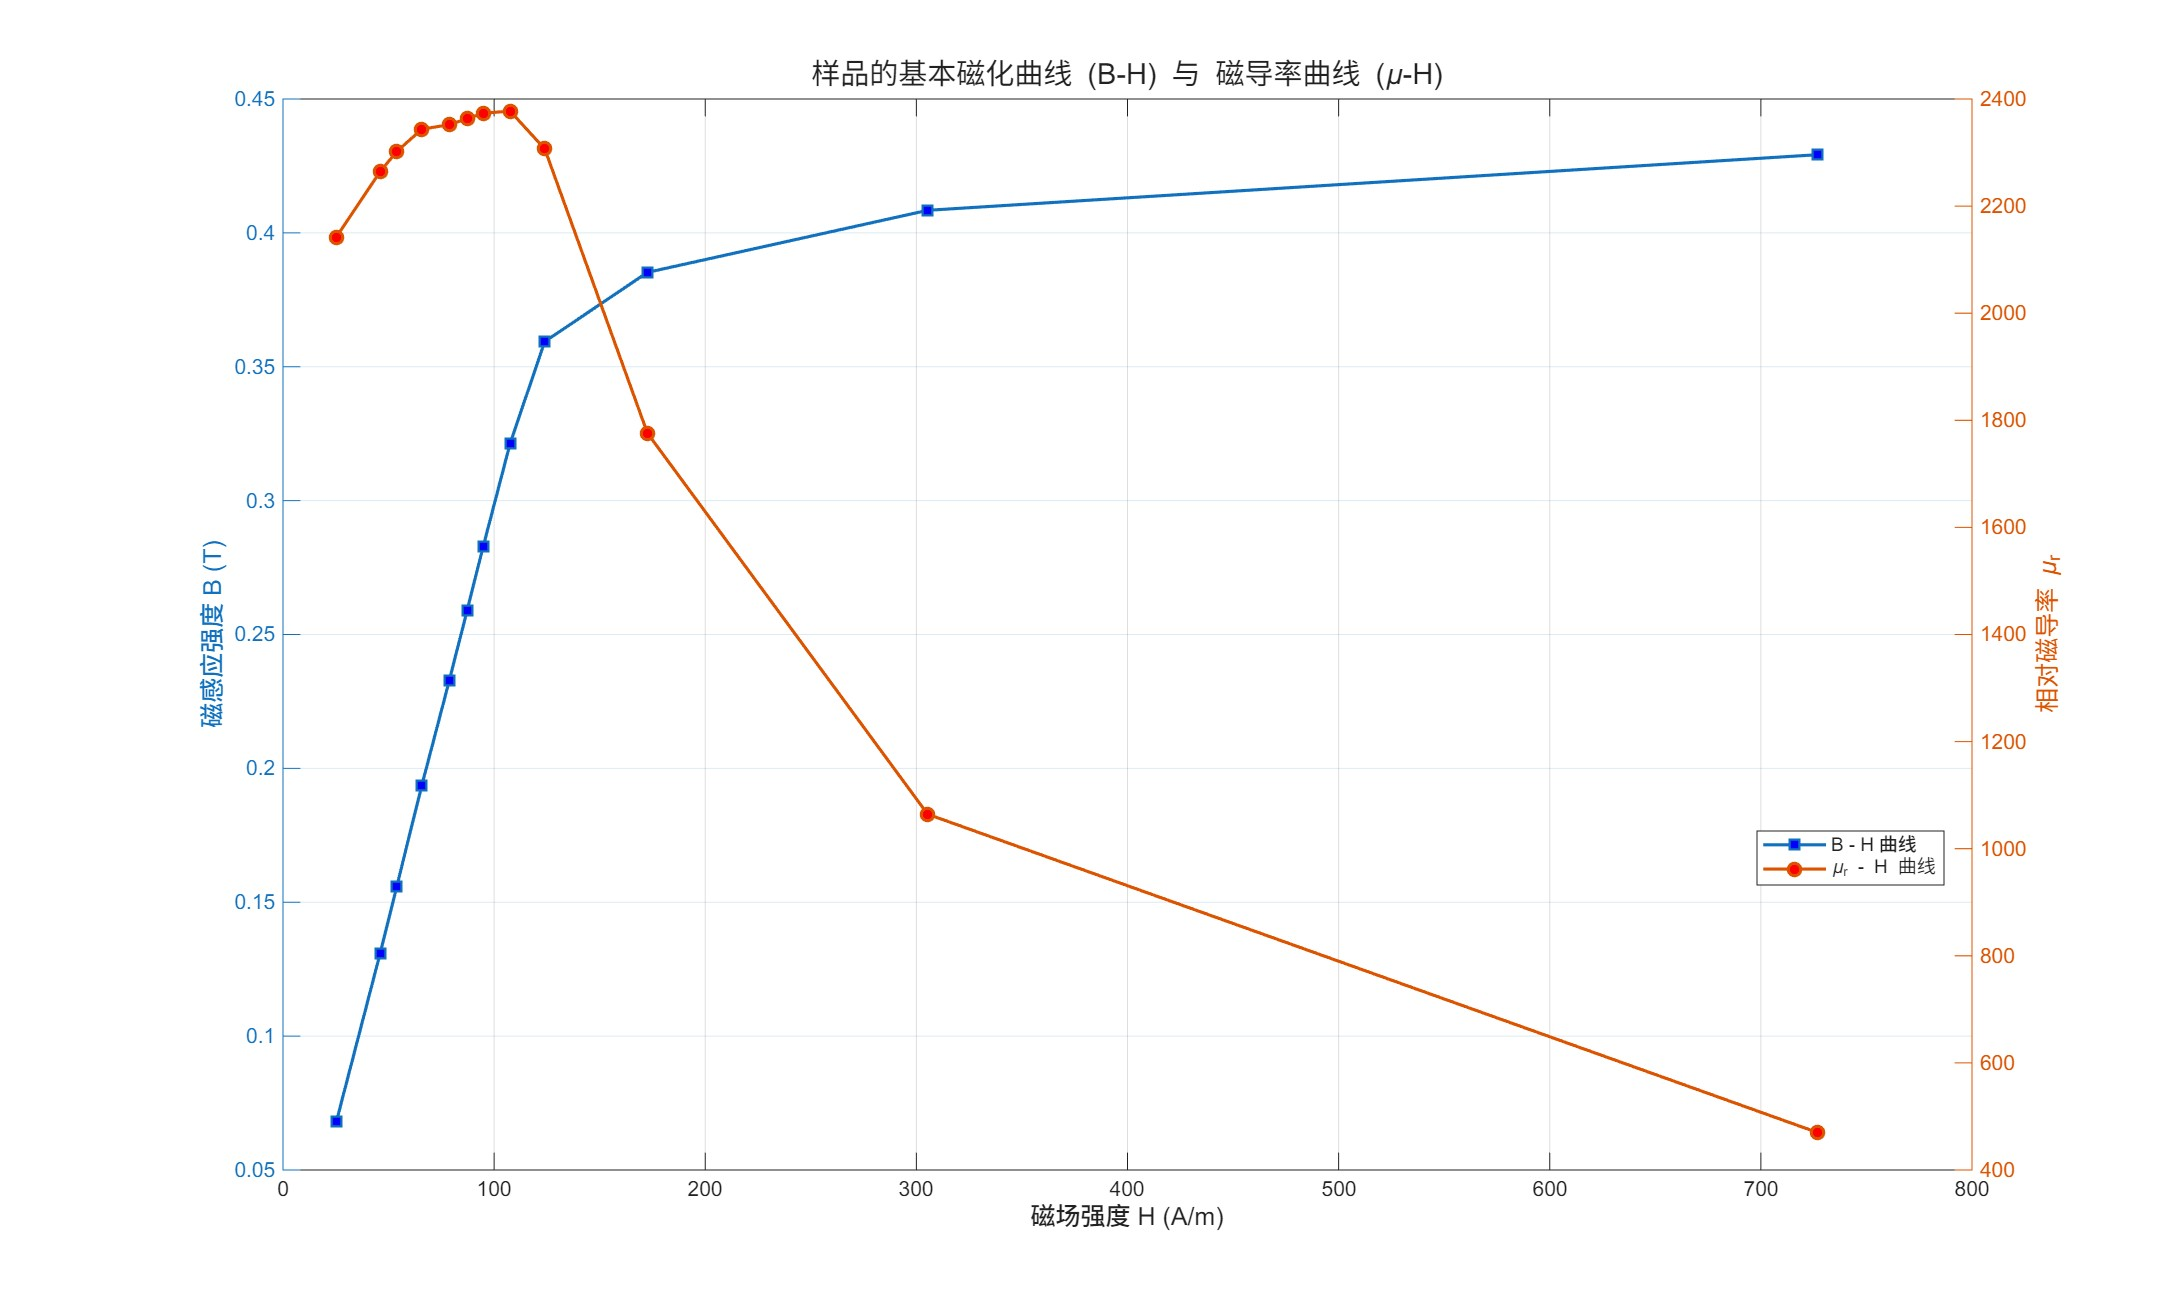
\includegraphics[width=0.8\textwidth]{figures/2/基本磁化曲线.jpg}
        \caption{样品的基本磁化曲线 ($B-H$) 与 磁导率曲线 ($\mu_r-H$)}
        \label{fig:basic_curve}
    \end{figure}

    \textbf{结果分析与物理意义：}

    观察基本磁化曲线可知，铁磁材料的磁化过程呈现明显的非线性特征。在磁场强度较弱的初始阶段，磁感应强度 $B$ 随外场 $H$ 的增加而急剧上升，这是因为材料内部的磁畴壁在外场作用下发生了不可逆的位移和合并。当磁场强度进一步增大至约 \SI{110}{\ampere\per\meter} 时，曲线斜率达到最大，对应的相对磁导率 $\mu_r$ 也达到峰值约 2376，表明此时材料的导磁性能最强。

    随着磁场继续增强， $B$ 的增长趋于平缓。当外加电压超过 \SI{3.0}{\volt} 后，即便励磁电流大幅增加导致 $H$ 激增至 \SI{700}{\ampere\per\meter} 以上，磁感应强度 $B$ 仅维持在 \SI{0.43}{\tesla} 左右并趋于定值。这一现象清晰地展示了铁磁材料的磁饱和特性。

    \subsubsection{磁滞回线测量}

    在固定外加电压的情况下，我们逐点记录了示波器显示的磁滞回线波形数据。表 \ref{tab:hysteresis_data} 展示了修正后的电压读数以及对应的磁场强度 $H$ 和磁感应强度 $B$。

    \begin{table}[H]
        \centering
        \caption{磁滞回线原始数据与换算结果}
        \label{tab:hysteresis_data}
        \scriptsize
        \setlength{\tabcolsep}{2pt} % 稍微减小列间距以适应增加的列
        \begin{tabularx}{\textwidth}{cXXXX|cXXXX}
            \toprule
            序号 & $U_x$ (\unit{\volt}) & $U_y$ (\unit{\volt}) & $H$ (\unit{\ampere\per\meter}) & $B$ (\unit{\tesla}) & 序号 & $U_x$ (\unit{\volt}) & $U_y$ (\unit{\volt}) & $H$ (\unit{\ampere\per\meter}) & $B$ (\unit{\tesla}) \\
            \midrule
            1  & -0.284               & -0.226               & -65.63                         & -0.182              & 17 & 0.178                & 0.216                & 41.08                          & 0.174               \\
            2  & -0.275               & -0.215               & -63.55                         & -0.173              & 18 & 0.302                & 0.225                & 69.76                          & 0.181               \\
            3  & -0.267               & -0.196               & -61.50                         & -0.158              & 19 & 0.273                & 0.195                & 62.98                          & 0.157               \\
            4  & -0.263               & -0.141               & -60.60                         & -0.113              & 20 & 0.263                & 0.122                & 60.60                          & 0.098               \\
            5  & -0.256               & -0.096               & -59.12                         & -0.077              & 21 & 0.259                & 0.097                & 59.72                          & 0.078               \\
            6  & -0.246               & -0.041               & -56.77                         & -0.033              & 22 & 0.247                & 0.045                & 57.05                          & 0.036               \\
            7  & -0.231               & 0.000                & -53.22                         & 0.000               & 23 & 0.232                & 0.000                & 53.52                          & 0.000               \\
            8  & -0.222               & 0.015                & -51.14                         & 0.012               & 24 & 0.208                & -0.041               & 47.88                          & -0.033              \\
            9  & -0.200               & 0.050                & -46.11                         & 0.040               & 25 & 0.176                & -0.080               & 40.50                          & -0.064              \\
            10 & -0.165               & 0.084                & -38.12                         & 0.068               & 26 & 0.122                & -0.125               & 28.08                          & -0.101              \\
            11 & -0.122               & 0.120                & -28.08                         & 0.097               & 27 & 0.087                & -0.145               & 20.12                          & -0.117              \\
            12 & -0.051               & 0.158                & -11.83                         & 0.127               & 28 & 0.000                & -0.182               & 0.00                           & -0.147              \\
            13 & 0.000                & 0.178                & 0.00                           & 0.143               & 29 & -0.024               & -0.189               & -5.62                          & -0.152              \\
            14 & 0.062                & 0.195                & 14.19                          & 0.157               & 30 & -0.091               & -0.205               & -20.99                         & -0.165              \\
            15 & 0.079                & 0.200                & 18.33                          & 0.161               & 31 & -0.174               & -0.218               & -40.20                         & -0.176              \\
            16 & 0.141                & 0.209                & 32.52                          & 0.169               & 32 & -0.231               & -0.225               & -53.33                         & -0.181              \\
            \bottomrule
        \end{tabularx}
    \end{table}

    依据表 \ref{tab:hysteresis_data} 中的数据，使用 Matlab 进行了绘图，绘制出平滑的磁滞回线图，并计算了相关的磁学参数。

    \begin{figure}[H]
        \centering
        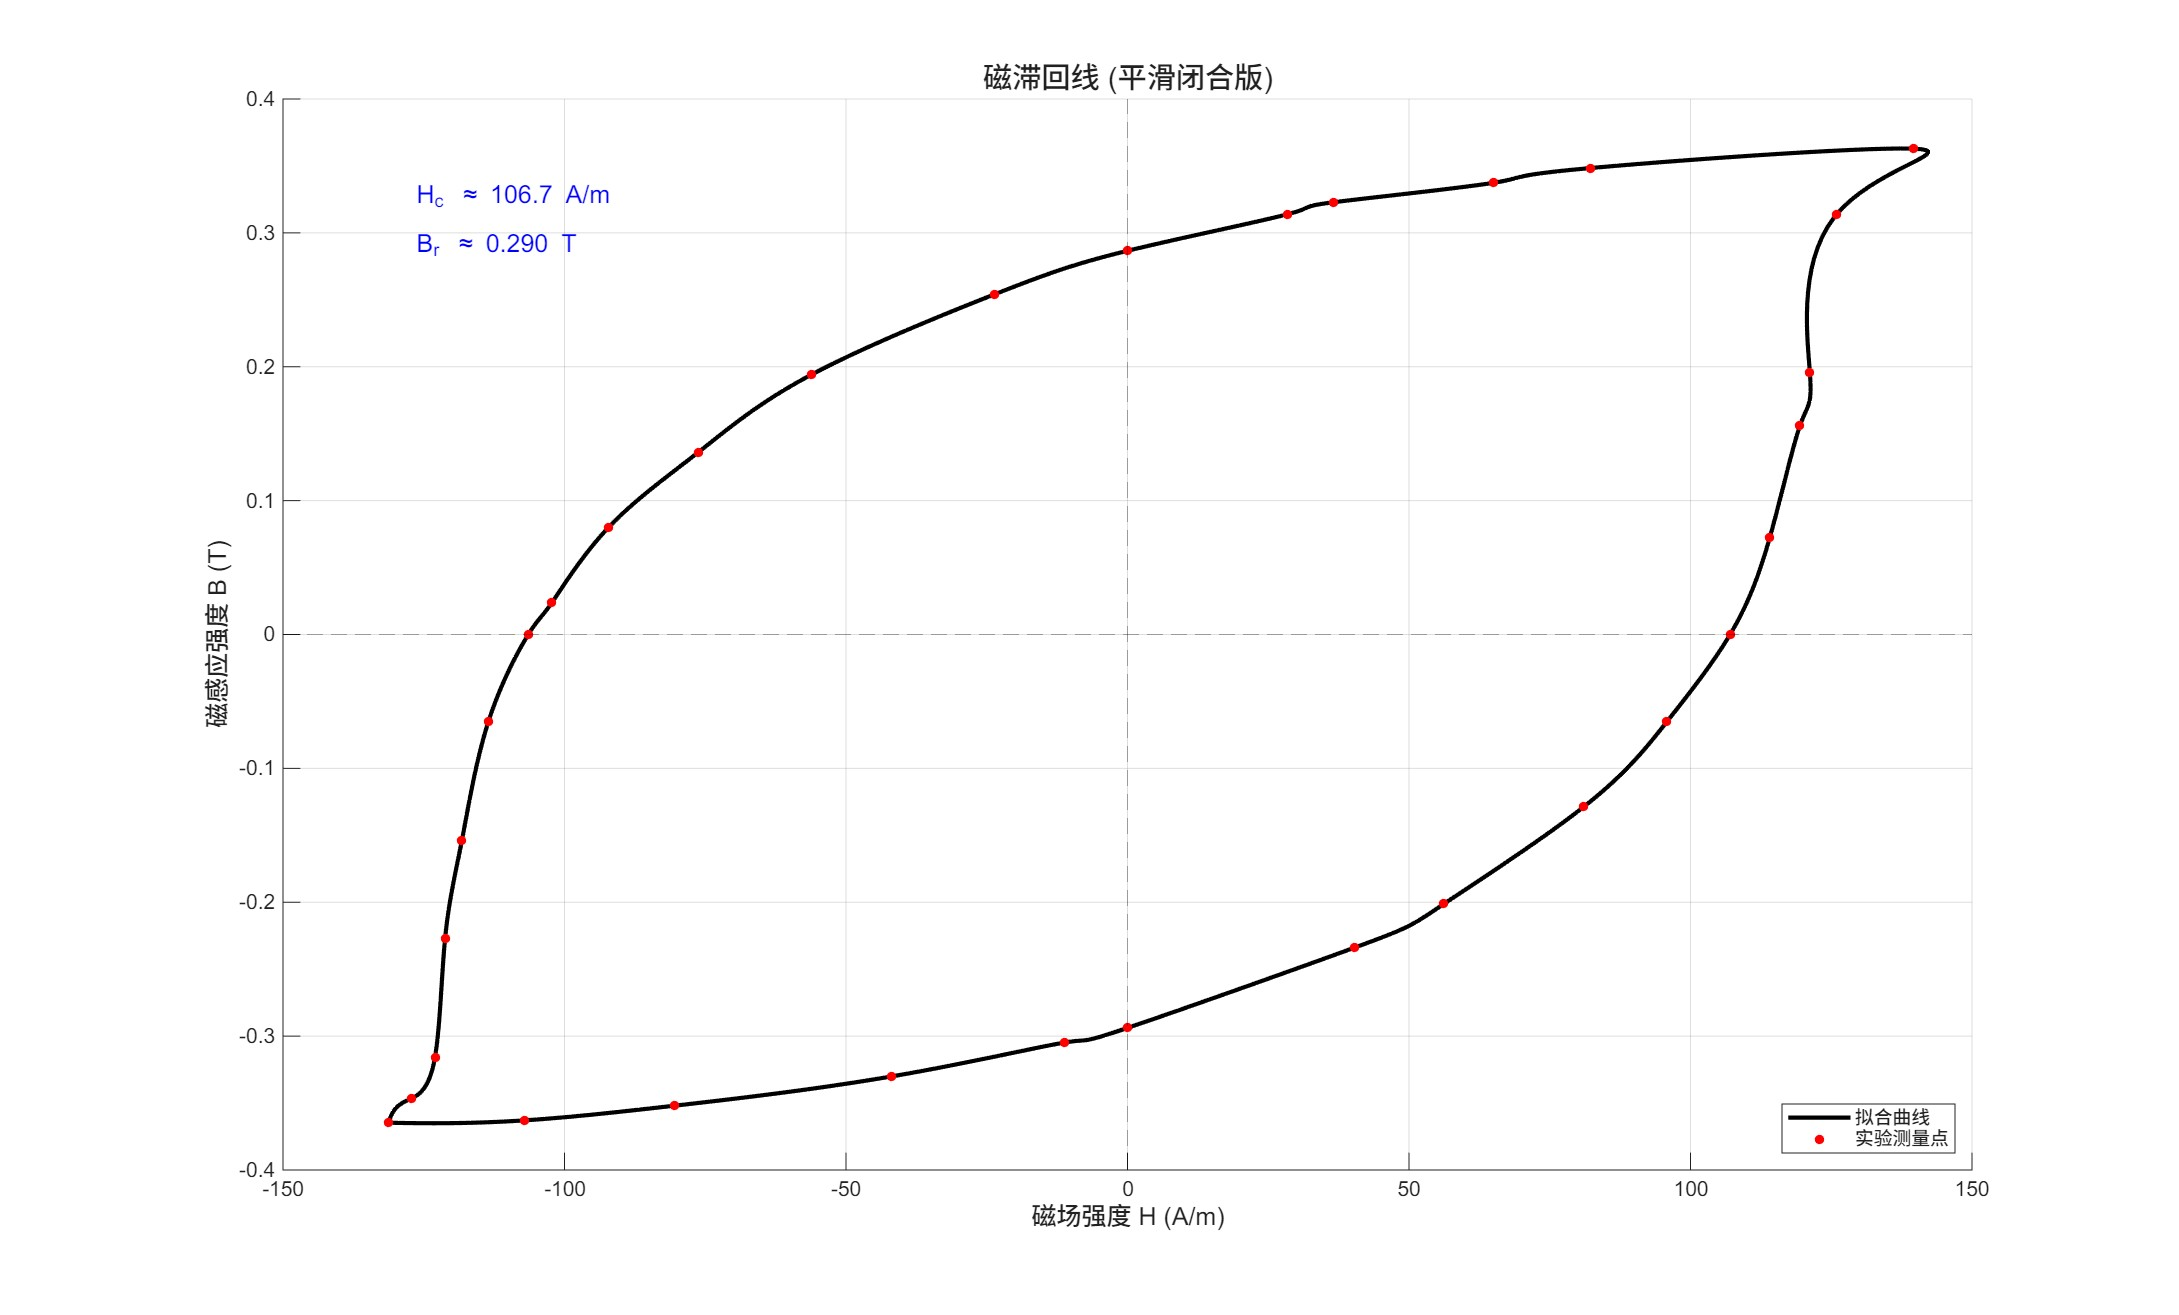
\includegraphics[width=0.7\textwidth]{figures/2/磁滞回线.jpg}
        \caption{实验测得的动态磁滞回线}
        \label{fig:hysteresis_loop}
    \end{figure}

    \textbf{磁参数计算与物理意义分析：}

    通过对磁滞回线数据的分析，我们提取了以下关键参数：
    \begin{itemize}
        \item \textbf{饱和磁感应强度} $B_m \approx \SI{0.365}{\tesla}$：这是材料在实验外场下所能达到的最大磁感应强度，反映了材料的磁化能力上限。
        \item \textbf{矫顽力} $H_c \approx \SI{106.7}{\ampere\per\meter}$：即当磁感应强度 $B$ 降为零时所需的反向磁场强度。该数值较低，表明实验所用的材料属于软磁材料，易于磁化也易于退磁。
        \item \textbf{剩磁} $B_r \approx \SI{0.290}{\tesla}$：当外加磁场完全撤去（$H=0$）时，材料内部仍保留的磁感应强度，体现了材料的磁记忆特性。
        \item \textbf{磁滞损耗} $W_h \approx \SI{119.0}{\joule\per\meter\cubed}$：即磁滞回线所包围的面积。这一数值代表材料在交变磁场中磁化一周单位体积所消耗的能量，该能量最终转化为热能。
    \end{itemize}

    磁滞回线的形成本质上是磁化过程不可逆性的宏观表现。当外磁场周期性变化时，磁畴壁的钉扎效应和不可逆位移导致 $B$ 的变化总是滞后于 $H$ 的变化，从而形成闭合回路。
    本实验测得的回线狭长，矫顽力小且磁滞损耗低，符合变压器铁芯等应用对软磁材料低损耗特性的要求。

    \subsection{误差分析}

    本次实验的误差主要来源于以下几个方面。首先是读数误差，由于使用模拟示波器或从数字示波器截图中手动读取光标位置，人眼的判断会引入随机误差，尤其是在波形变化陡峭的区域。

    其次是仪器误差，实验箱内部的采样电阻 $R_1$ 和积分电容 $C$ 存在标称公差，这会直接影响转换系数 $K$ 的准确性，导致计算出的 $H$ 和 $B$ 值存在系统误差。

    \subsection{实验探讨}

    通过本次实验，我们不仅掌握了利用示波器观测动态磁滞回线的实验方法，更从物理图像上直观理解了铁磁材料的磁化特性。实验结果表明，磁导率 $\mu$ 并非通过简单的线性关系得出，而是一个随磁场强度剧烈变化的非线性参量。

    在数据处理过程中，我们发现示波器探头衰减设置对测量结果有显著影响，必须正确处理探头系数才能还原真实的物理量。

    此外，通过对比不同电压下的回线形状，我们深刻体会到只有在足够强的外场下，材料才能达到深度饱和，从而测得完整的磁参数。

    \section{思考题}

    \subsection{\texorpdfstring{$\mathrm{B} \cdot \mathrm{H}$}{B·H}（磁能积）的单位是否与能量有关? 请给出量纲的推导过程。}
    磁能积 $(BH)_{max}$ 的单位直接对应着能量密度。

    磁感应强度 $B$ 的定义式为 $F = qvB$，其量纲可表示为 \unit{\newton\per\ampere\per\meter}；磁场强度 $H$ 根据安培环路定理定义，其量纲为 \unit{\ampere\per\meter}。将两者相乘，电流单位 \unit{\ampere} 相互抵消，得到 $B \cdot H$ 的量纲为 \unit{\newton\per\meter\squared}。在物理学中，\unit{\newton\cdot\meter} 等价于能量单位焦耳 \unit{\joule}，因此 \unit{\newton\per\meter\squared} 可以上下同乘米得到 \unit{\joule\per\meter\cubed}。
    这表明磁能积在物理意义上代表了单位体积内的磁场能量，即能量密度，常用于衡量永磁体对外做功的能力。

    \subsection{查阅有关资料，简要回答积分电路的原理与有关应用}
    积分电路本质上是一个由电阻 $R$ 和电容 $C$ 构成的线性网络，
    其输出电压 $V_{out}$ 与输入电压 $V_{in}$ 的时间积分成正比，即 $V_{out} \propto \int V_{in} dt$。
    在本实验中，积分电路扮演着至关重要的信号转换角色。
    由于探测线圈测量的是感应电动势 $E \propto -\frac{dB}{dt}$，该信号正比于磁感应强度的变化率而非 $B$ 本身。
    为了在示波器上直接观测 $B$ 的波形，必须让感应电动势信号通过积分电路，还原出与 $B$ 成正比的电压信号 $U_y$。这利用了积分运算是微分运算的逆运算原理，从而实现了从 $\frac{\mathrm{d}B}{\mathrm{d}t}$ 到 $B$ 的物理量转换。

    \subsection{磁性材料内部的涡流损耗的能量是否可以被利用起来?请列出应用实例。}
    虽然涡流损耗在变压器和电机中浪费了许多能量，但在特定场合下，我们完全可以利用这种将电磁能转化为热能或机械阻尼的效应。

    生活中最常见的例子是电磁炉，它利用交变磁场在铁磁性锅底产生强大的涡流，利用涡流的热效应迅速加热食物。

    另一个重要的应用是电磁制动，例如新能源电车或者高速列车，通过在导轨或刹车盘上感生涡流，利用楞次定律产生的反向电磁力将动能转化为涡流热能耗散掉，从而实现非接触式的平稳减速。
\end{fullreportonly}
\insertnotes
\end{document}